\documentclass[a4paper,12pt]{article}
%%%%%%%%%%%%%%%%%%%%%%%%%%%%%%%%%%%%%%%%%%%%%%%%%%%%%%%%%%%%%%%%%%%%%%%%%%%%%%%%%%%%%%%%%%%%%%%%%%%%%%%%%%%%%%%%%%%%%%%%%%%%%%%%%%%%%%%%%%%%%%%%%%%%%%%%%%%%%%%%%%%%%%%%%%%%%%%%%%%%%%%%%%%%%%%%%%%%%%%%%%%%%%%%%%%%%%%%%%%%%%%%%%%%%%%%%%%%%%%%%%%%%%%%%%%%
\usepackage{eurosym}
\usepackage{vmargin}
\usepackage{amsmath}
\usepackage{graphics}
\usepackage{epsfig}
\usepackage{framed}
\usepackage{subfigure}
\usepackage{fancyhdr}

\setcounter{MaxMatrixCols}{10}
%TCIDATA{OutputFilter=LATEX.DLL}
%TCIDATA{Version=5.00.0.2570}
%TCIDATA{<META NAME="SaveForMode"CONTENT="1">}
%TCIDATA{LastRevised=Wednesday, February 23, 201113:24:34}
%TCIDATA{<META NAME="GraphicsSave" CONTENT="32">}
%TCIDATA{Language=American English}

\pagestyle{fancy}
\setmarginsrb{20mm}{0mm}{20mm}{25mm}{12mm}{11mm}{0mm}{11mm}
\lhead{MA4128} \rhead{Kevin O'Brien} \chead{Linear Models} %\input{tcilatex}

%http://www.electronics.dit.ie/staff/ysemenova/Opto2/CO_IntroLab.pdf
\begin{document}



\section{Linear Regression Analysis}

\subsection{Introduction}
\begin{itemize}
	\item Linear regression is used when you want to predict the value of a variable based on the value of another variable.
	\begin{itemize}
	\item[$\ast$] The variable we want to predict is called the \textbf{\textit{dependent variable}} (or the response variable or outcome variable). 
	\item[$\ast$] The variable we are using to predict the other variable's value is called the \textbf{\textit{independent variable}} (or the predictor variable).
	\end{itemize}
	
\item For example, you could use linear regression to understand whether exam performance can be predicted based on revision time; whether cigarette consumptions can be predicted based on smoking duration; and so forth. If you have two or more independent variables, rather than just one, you need to use \textbf{\textit{multiple regression}}.
	
\item SPSS can be used to carry out linear regression, as well as interpret and report the results from this test. However, before we introduce you to this procedure, you need to understand the different assumptions that your data must meet in order for linear regression to give you a valid result. We discuss these assumptions next.
\end{itemize}



\subsection{Assumptions}
When you choose to analyse your data using linear regression, part of the process involves checking to make sure that the data you want to analyse can actually be analysed using linear regression. You need to do this because it is only appropriate to use linear regression if your data is appropriate for six assumptions that are required for linear regression to give you a valid result.

In practice, checking for these six assumptions just adds a little bit more time to your analysis, requiring you to click a few more buttons in SPSS when performing your analysis, as well as think a little bit more about your data, but it is not a difficult task.

Often when analysing your own data using SPSS, one or more of these assumptions is violated (i.e., not met). This is not uncommon when working with real-world data rather than textbook examples, which often only show you how to carry out linear regression when everything goes well. However, even when your data fails certain assumptions, there is often a solution to overcome this. First, let’s take a look at these six assumptions:

\begin{itemize}
\item \textbf{Assumption 1}: Your two variables should be measured at the interval or ratio level (i.e., they are continuous). Examples of variables that meet this criterion include revision time (measured in hours), intelligence (measured using IQ score), exam performance (measured from 0 to 100), weight (measured in kg), and so forth. 

\item \textbf{Assumption 2}: There needs to be a linear relationship between the two variables. Whilst there are a number of ways to check whether a linear relationship exists between your two variables, we suggest creating a scatter-plot using SPSS, where you can plot the dependent variable against your independent variable, and then visually inspect the scatter-plot to check for linearity. Your scatter-plot may look something like one of the following:



\begin{figure}[h!]
\begin{centering}
  % Requires \usepackage{graphicx}
  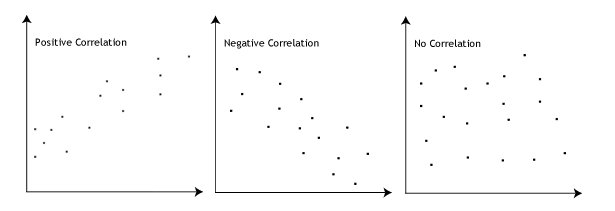
\includegraphics[width=12cm]{Regre1.jpg}\\
  \caption{Types of Linear Relationship}
\end{centering}
\end{figure}
If the relationship displayed in your scatterplot is not linear, you will have to either run a non-linear regression analysis or \textbf{\textit{transform}} your data, which you can do using SPSS. It is important to learn how to:
\begin{itemize}
	\item[(a)] create a scatterplot to check for linearity when carrying out linear regression using SPSS; 
	\item[(b)] interpret different scatterplot results; 
	\item[(c)] transform your data using SPSS if there is not a linear relationship between your two variables.
\end{itemize} 


\item \textbf{Assumption 3}: There should be no significant outliers. Outliers are simply single data points within your data that do not follow the usual pattern (e.g., in a study of 100 students’ IQ scores, where the mean score was 108 with only a small variation between students, one student had a score of 156, which is very unusual, and may even put her in the top 1\% of IQ scores globally). The following scatterplots highlight the potential impact of outliers:

The problem with outliers is that they can have a negative effect on the regression equation that is used to predict the value of the dependent (outcome) variable based on the independent (predictor) variable. This will change the output that SPSS produces and reduce the predictive accuracy of your results. Fortunately, when using SPSS to run linear regression on your data, you can easily include criteria to help you detect possible outliers.
\begin{figure}[h!]
\begin{centering}
  % Requires \usepackage{graphicx}
  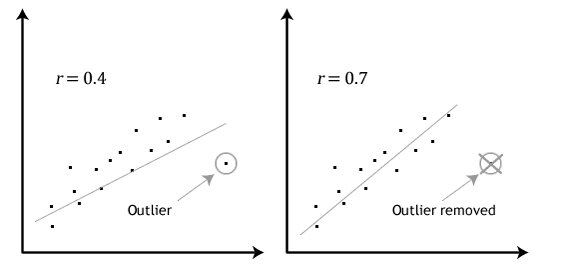
\includegraphics[width=12cm]{Regre2.jpg}\\
  \caption{Effect of an Outlier}
\end{centering}
\end{figure}
%In our enhanced linear regression guide, we: (a) show you how to detect outliers using \textbf{case-wise diagnostics}, which is a simple process when using SPSS; and (b) discuss some of the options you have in order to deal with outliers.
\item \textbf{Assumption 4}: You should have independence of observations, which you can easily check using the Durbin-Watson statistic, which is a simple test to run using SPSS. An explantion on how to interpret the result of the Durbin-Watson statistic will be discussed later.

\item \textbf{Assumption 5}:Your data needs to show \textbf{\textit{homoscedasticity}}, which is where the variances along the line of best fit remain similar as you move along the line. Whilst we explain more about what this means and how to assess the homoscedasticity of your data in the linear regression line, take a look at the two scatter-plots below, which provide two simple examples: one of data that meets this assumption and one that fails the assumption:

\begin{figure}[h!]
\begin{centering}
  % Requires \usepackage{graphicx}
  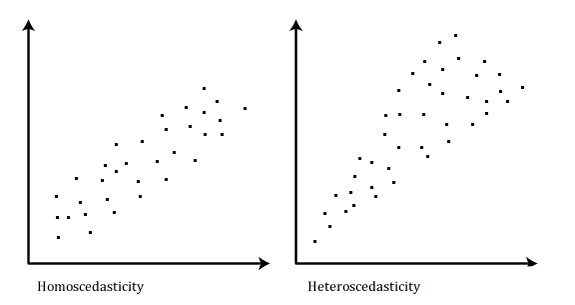
\includegraphics[width=12cm]{Regre3.jpg}\\
  \caption{Constant Variance}
\end{centering}
\end{figure}
When you analyse your own data, you will be lucky if your scatterplot looks like either of the two above. Whilst these help to illustrate the differences in data that meets or violates the assumption of homoscedasticity, real-world data is often a lot more messy.

% Therefore, in our enhanced linear regression guide, we explain: (a) some of the things you will need to consider when interpreting your data; and (b) possible ways to continue with your analysis if your data fails to meet this assumption.

\item \textbf{Assumption 6}:Finally, you need to check that the residuals (errors) of your two variables are approximately normally distributed. Two common methods to check this assumption include using either a histogram (with a superimposed normal curve) or by using a Normal Probability Plot.
  %  Again, in our enhanced linear regression guide, we: (a) show you how to check this assumption using SPSS, whether you use a histogram (with superimposed normal curve) or Normal P-P Plot; (b) explain how to interpret these diagrams; and (c) provide a possible solution if your data fails to meet this assumption.

\end{itemize}
You can check assumptions all assumptions except no.1 using SPSS. It is recommended to test these assumptions in this order because it represents an order where, if a violation to the assumption is not correctable, you will no longer be able to use a single linear regression (although you may be able to run another statistical test on your data instead). Just remember that if you do not run the statistical tests on these assumptions correctly, the results you get when running a linear regression might not be valid.


\newpage

\section{Output of Linear Regression Analysis}
Linear regression is used when you want to predict the value of a variable based on the value of another variable. The variable we want to predict is called the dependent variable (or sometimes, the outcome variable). The variable we are using to predict the other variable's value is called the independent variable (or sometimes, the predictor variable).
\[ \hat{y} = b_o + b_1 x \]
\begin{itemize}
\item $b_o$ is the intercept estimate
\item $b_1$ is the slope estimate
\item $\hat{y}$ is the \textbf{\textit{fitted}} y-value, given a specified value of the indepenent variable $x$.
\item The fitted value and the observed value of y often differ. This difference is known as the \textbf{\textit{residual}}
\end{itemize}

For example, you could use linear regression to understand whether exam performance can be predicted based on revision time; whether cigarette consumptions can be predicted based on smoking duration; and so forth. If you have two or more independent variables, rather than just one, you need to use \textbf{\textit{multiple regression}}.

SPSS will generate quite a few tables of output for a linear regression procedure. Only the three main tables required to understand your results from the linear regression procedure, assuming that no assumptions have been violated.

This includes relevant scatterplots, histogram (with superimposed normal curve) and Normal Probability Plot (i.e. Q-Q plots), and case-wise diagnostics and Durbin-Watson statistic tables. Below, we focus on the results for the linear regression analysis only.

\begin{figure}[h!]
\begin{centering}
  % Requires \usepackage{graphicx}
  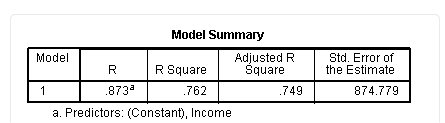
\includegraphics[width=15cm]{Regre4.jpg}\\
 % \caption{Model Summary table}
\end{centering}
\end{figure}

The first table of interest is the \textbf{\textit{Model Summary}} table. This table provides the R and $R^2$ value. The R value is 0.873, which represents the simple correlation. It indicates a high degree of correlation. The $R^2$ value indicates how much of the dependent variable, \textbf{\textit{price}} (Not evident on output), can be explained by the independent variable,\textbf{\textit{income}}. In this case, 76.2\% can be explained, which is very large.


The next table is the ANOVA table. This table indicates that the regression model predicts the outcome variable significantly well. How do we know this? Look at the \textbf{\textit{Regression}} row and go to the \textbf{Sig.} column. This indicates the statistical significance of the regression model that was applied. Here,the p-value is  $p < 0.0005$, which is less than 0.05, and indicates that, overall, the model applied can statistically significantly predict the outcome variable.

\begin{figure}[h!]
\begin{centering}
  % Requires \usepackage{graphicx}
  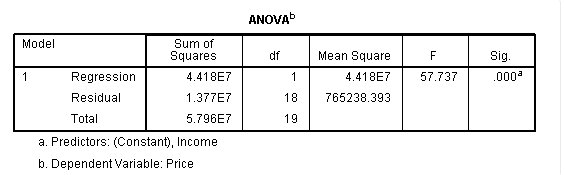
\includegraphics[width=15cm]{Regre5.jpg}\\
%  \caption{ANOVA Table}
\end{centering}
\end{figure}

The next table again, \textbf{\textit{Coefficients}}, provides us with information on each predictor variable. This gives us the information we need to predict price from income. We can see that both the constant and income contribute significantly to the model (by looking at the \texttt{Sig.} column). 

By looking at the B column under the \texttt{Unstandardized Coefficients} column, we can present the regression equation as:
\begin{center}
\textit{\textbf{ $\hat{Price}$ = 8287 + 0.564(Income)}}
\end{center}
\begin{figure}[h!]
\begin{centering}
  % Requires \usepackage{graphicx}
  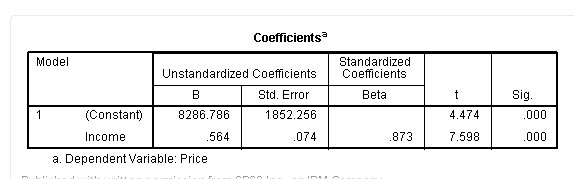
\includegraphics[width=15cm]{Regre6.jpg}\\
  %\caption{Coefficients Table}
\end{centering}
\end{figure}


\newpage

\subsection{What is Multiple Linear Regression}

Multiple regression is a statistical technique that allows us to predict a numeric value on the response variable on the basis of the observed values on several other independent variables.


\[\hat{y} = b_0 + b_1x_1 + b_2x_2 + \ldots \]

\begin{itemize}
	\item $\hat{y}$ is the \textbf{\textit{fitted value}} for the dependent variable \textbf{$Y$}, given a linear combination of values for the independent valriables.
	
	\item $x_i$ is the value for independent variable \textbf{$X_i$}. (For Example, $x_1$ is the value for independent variable \textbf{$X_1$}.)
	\item $b_o$ is the constant regression estimate ( commonly known as the \textbf{Intercept Estimate} in the case of simple linear regression).
	\item $b_i$ is the regression estimate for Independent Variable \textbf{$X_1$} ( commonly known as the \textbf{Slope Estimate} in the case of simple linear regression).
\end{itemize}

\subsubsection{Simple Example}
Suppose we were interested in predicting how much an individual enjoys their job. Independent Variables such as salary, extent of academic qualifications, age, sex, number of years in full-time employment and socioeconomic status might all contribute towards \textbf{\textit{job satisfaction}}.

If we collected data on all of these variables, perhaps by surveying a few hundred members of the public, we would be able to see how many and which of these variables gave rise to the most accurate prediction of job satisfaction. We might find that job satisfaction is most accurately predicted by type of occupation, salary and years in full-time employment, with the other variables not helping us to predict job satisfaction.


%-----------------------------------------------------------------------------------------%
\section{Multiple Linear Regression}
Multiple regression: To quantify the relationship between several independent (predictor) variables and a dependent (response) variable. The coefficients ($a, b_{1} to b_{i}$) are estimated by the least squares method, which is equivalent to maximum likelihood estimation. A multiple regression model is built upon three major assumptions:

\begin{enumerate}
	\item The response variable is normally distributed,
	\item The residual variance does not vary for small and large fitted values (constant variance),
	\item The observations (explanatory variables) are independent.
\end{enumerate}


\subsection{Dummy Variables}
A dummy variable is a numerical variable used in regression analysis to represent subgroups of the sample in your study. In research design, a dummy variable is often used to distinguish different treatment groups. In the simplest case, we would use a 0,1 dummy variable where a person is given a value of 0 if they are in the control group or a 1 if they are in the treated group. Dummy variables are useful because they enable us to use a single regression equation to represent multiple groups. This means that we don't need to write out separate equation models for each subgroup.



\end{document}
